\documentclass{article}
%%%%%%%%%%%%%%%%%%%%%%%%%
%%% PACKAGE INCLUSION %%%
%%%%%%%%%%%%%%%%%%%%%%%%%

%% AMS packages for special symbols, etc
\usepackage{amsmath,amssymb}

%% This package gives you coloured text and various other simple
%% graphics hacks.  For details, see documentation in 
%% in /usr/local/teTeX/texmf/doc/generic/pstricks/*
\usepackage{pstricks}
\newrgbcolor{darkblue}{0.1 0.1 0.5}

%% The textpos package is necessary to position textblocks at arbitary 
%% places on the page.  Use showboxes option to show outlines of textboxes.
\usepackage[absolute]{textpos}
%\usepackage[absolute,showboxes]{textpos}

%% Package to include graphics.  
\usepackage{graphicx}
%% Define path for figures -- for safety, keep the last /
\graphicspath{{/your/figure/directory/here/if/any/}
{/an/second/directory/path/can/go/here/}}

%% Wrap text around figures
%\usepackage{wrapfig}

%% Use Times font instead of Computer Modern -- this gives better
%% appearance when resizing to large sixes.
%% Note that without the ``G0'' in the dvips conversion, 
%% all character combinations that will normally result in 
%% ligatures will have to be hacked to display properly.  For example, 
%%     fi --> \mbox{f}\mbox{i}
%% Other characters may also fail.  In addition, the Mathtimes font 
%% set should really be used for mathematics, but unfortunately they 
%% are only proprietary.  (The Computer Modern fonts may still look OK.)
\usepackage{times}

%% These colors are tried and tested for titles and headers. Don't
%% over use color!
%\usepackage[usenames]{color} % commented by Karol Kozioł
\usepackage{xcolor}
\definecolor{DarkBlue}{rgb}{0.1,0.1,0.5}
\definecolor{Black}{rgb}{0.0,0.0,0.0}
\definecolor{Red}{rgb}{0.9,0.0,0.1}
\definecolor{DarkBlue2}{rgb}{0.00,0.08,0.6}
\definecolor{DarkRed2}{rgb}{0.6,0.00,0.08}
\definecolor{DarkGreen2}{rgb}{0.00,0.6,0.08}

%% Load shadow box package
%\usepackage{shadow}

%% This loads font sizes in style file a0size
\usepackage{a0size}

%%%%%%%%%%%%%%%%%%%%%%%%%%%%%%%% 
%%% NEW COMMAND DEFINTITIONS %%%
%%%%%%%%%%%%%%%%%%%%%%%%%%%%%%%%

%%    \normalsize will produce smaller type that might look too small
%%    \large will produce larger type
% \let\Textsize\normalsize
\let\Textsize\large
\def\RHead#1{\noindent\hbox to \hsize{\hfil{\LARGE\color{DarkBlue} #1}}\bigskip}
\def\LHead#1{\noindent{\LARGE\color{DarkBlue} #1}\bigskip}
\def\CHead#1{\begin{center}\noindent{\LARGE\color{DarkBlue} #1}\end{center}}
\def\Subhead#1{\noindent{\large\color{DarkBlue} #1}\bigskip}
\def\Title#1{\noindent{\textbf{\veryHuge\color{Red} #1}}}

%%%%%%%%%%%%%%%%%%%%%%%%%%%%%
%%% GLOBAL LAYOUT OPTIONS %%%
%%%   NUMBER OF COLUMNS   %%%
%%%%%%%%%%%%%%%%%%%%%%%%%%%%%

%% Set paper size
%% Depending on the conference, the posterboard size may be different.
%% This template was based on an ISO standard A0, which is in use everywhere
%% except for the United States.  A0 paper is  46.81 in x 33.11 in.
%% Depending on the posterboard size and the printer, you may need to 
%% change the widths and margins here.  Text width and height are set
%% in terms of paper width and height -- you can change margins here.
\setlength{\paperwidth}{40in}
\setlength{\paperheight}{30in}
\setlength{\textwidth}{36in}    %% paperwidth - (3in)
\setlength{\textheight}{26in}   %% paperheight - (3in)
\special{papersize=\the\paperwidth,\the\paperheight}
\typeout{Paper width and height are \the\paperwidth and \the\paperheight}
\typeout{Text width and height are \the\textwidth and \the\textheight}
%% Margins
\setlength{\headheight}{0cm}
\setlength{\headsep}{0cm}
\setlength{\topmargin}{1in}
\setlength{\topskip}{0cm}
\setlength{\oddsidemargin}{1in}
\setlength{\evensidemargin}{0in}
%% Font sizes
\renewcommand{\tiny}{\fontsize{12}{14}\selectfont}
\renewcommand{\scriptsize}{\fontsize{14.4}{18}\selectfont}   
\renewcommand{\footnotesize}{\fontsize{17.28}{22}\selectfont}
\renewcommand{\small}{\fontsize{20.74}{25}\selectfont}
\renewcommand{\normalsize}{\fontsize{24.88}{30}\selectfont}
\renewcommand{\large}{\fontsize{29.86}{37}\selectfont}
\renewcommand{\Large}{\fontsize{35.83}{45}\selectfont}
\renewcommand{\LARGE}{\fontsize{43}{54}\selectfont}
\renewcommand{\huge}{\fontsize{51.6}{64}\selectfont}
\renewcommand{\Huge}{\fontsize{61.92}{77}\selectfont}
\newcommand{\veryHuge}{\fontsize{74.3}{93}\selectfont}
\newcommand{\VeryHuge}{\fontsize{89.16}{112}\selectfont}
\newcommand{\VERYHuge}{\fontsize{107}{134}\selectfont}
%% skip lengths
\setlength{\smallskipamount}{6pt plus 2pt minus 2pt}
\setlength{\medskipamount}{12pt plus 4pt minus 4pt}
\setlength{\bigskipamount}{24pt plus 8pt minus 8pt}
\setlength{\abovecaptionskip}{25pt}
\setlength{\belowcaptionskip}{0pt}
\setlength{\abovedisplayskip}{25pt plus 6pt minus 15 pt}
\setlength{\abovedisplayshortskip}{0pt plus 6pt}
\setlength{\belowdisplayshortskip}{13pt plus 7pt minus 6pt}
\setlength{\belowdisplayskip}{\abovedisplayskip}

%% Set up the grid
%%
%% Note that [40mm,40mm] is the margin round the edge of the page
%% it is _not_ the grid size. That is always defined as 
%% PAGE_WIDTH/HGRID and PAGE_HEIGHT/VGRID. In this case we use
%% 46 x 26. This gives us 4 columns of width 10 boxes, with a gap of
%% width 2 in between them.  There are 26 vertical boxes.
%%
%% (Note however that texblocks can be positioned fractionally as well,
%% so really any convenient grid size can be used.)
%%
\TPGrid[40mm,40mm]{46}{26}      % 4 cols of width 10, plus 3 gaps width 2

%% Text layout parameters
\parindent=0pt
\parskip=0.5\baselineskip





%%%%%%%%%%%%%%%%%%%%%
%%% THEOREMS, ETC %%%
%%%%%%%%%%%%%%%%%%%%%
\newtheorem{thm}{Theorem}






%%%%%%%%%%%%%%%%%%%%%%%%%%%%
%%% DOCUMENT BEGINS HERE %%%
%%%%%%%%%%%%%%%%%%%%%%%%%%%%

%% The basic format of the poster is to create text boxes with the
%% various things you want to display.  You can then play around 
%% with how to lay thing out.  In the old version of this template,
%% the content was always provided with alternatives suitable for
%% printing on sheets of paper (resizing fonts, images, etc).  I
%% think that's too confusing to read.  The old layout was:
%%     \ifposter
%%          some poster commands go here
%%     \else
%%          an alternative style here in case you are printing on
%%          regular sheets of paper
%%     \fi
%% One option is to make the entire poster and then wrap it in an \ifposter
%% and then make all the slides separately.  This seems to be easier
%% if your poster is not much like a bunch of 8.5x11 sheet tacked together
%% in the first place.
\begin{document}

%% Do not put page numbers at the bottom of the page for poster
\pagestyle{empty}



%% Declare proper hyphenation
\hyphenation{equi-bi-ax-i-al}
\hyphenation{in-fin-i-tes-i-mal}


%% Border and background options -- you can make up others if you
%% like.  These all use the pstricks package.
%% DRAW A BLUE BORDER AROUND THE POSTER USING PSTRICKS
\psset{linewidth=0.5cm}
% Sets up lengths for frame
\newlength{\frameleft}
\newlength{\frameright}
\newlength{\frametop}
\newlength{\framebottom}
\setlength{\frameleft}{-1in}
\setlength{\frameright}{\textwidth}
\addtolength{\frameright}{1in}
\setlength{\frametop}{1in}
\setlength{\framebottom}{-\textheight}
\addtolength{\framebottom}{-1in}
% Draws a blue frame
\psframe[linecolor=darkblue,cornersize=absolute,linearc=2]
(\frameleft,\framebottom)(\frameright,\frametop)% need to overlay EOSMLS
%\psline{->}(0cm,0cm)(\textwidth,-\textheight)
%   *** End code to draw border *** 

%% USE A COLORED BACKGROUND FOR THE ENTIRE POSTER
%% [ADS 4-2005] THIS OPTION IS NOT SUPPORTED YET
%\newrgbcolor{gradbegin}{0.3 0.5 0.7}
%\newrgbcolor{LightBlue}{0.7 0.7 1.0}
%\psframe[fillstyle=solid,fillcolor=LightBlue](\frameleft,\framebottom)(\frameright,\frametop)



%% Adjust spacing in long displayed mathematical formulas to tighten them up
\setlength{\abovedisplayskip}{0.75\abovedisplayskip}
\setlength{\belowdisplayskip}{0.75\belowdisplayskip}



%% Understanding textblocks is the key to being able to do a poster in
%% LaTeX. The first argument gives the block width in grid cells, the
%% second gives the positioning on the grid.
%%
%% NOTE:  You will have to do a lot of previewing to get everything
%% in the right place.
%%
\begin{textblock}{46}(00,00)
\begin{center}
\Title{\LaTeX\ Template for Wireless Foundations Conference Posters v0.1}
\end{center}
\end{textblock}

\begin{textblock}{46}(00,01.5)
\begin{center}
\LHead{Anand D. Sarwate}\\
\LHead{\textit{Department of Electrical Engineering and Computer Sciences,
  University of California, Berkeley }}
\end{center}
\end{textblock}


%% UCB EECS logo on left, Wireless Foundations Logo on right
\begin{textblock}{8}(00.5,01)
\begin{center}
\includegraphics[height=5cm]{eecs.eps}
\end{center}
\end{textblock}

\begin{textblock}{8}(38,01)
\begin{center}
%
\includegraphics[height=5cm]{wifound.eps} % modified by Karol Kozioł

\includegraphics[height=2.5cm]{wifound.eps}
\end{center}
\end{textblock}


\begin{textblock}{42}(02,03)
\begin{center}
\rule{1200pt}{7pt}
\end{center}
\end{textblock}



%% Begin 1st row
\begin{textblock}{10}(00,04)
\CHead{Introduction}            %% \CHead creates a centered title
\begin{itemize}
\item The goal of this template is to give the conference posters
from Wireless Foundations a uniform ``look-and-feel.''
\item The source that created this document is a good place to
start if you are trying to make a conference poster or just want
to play around with the layout.
\item Since there are very few WYSIWYG \LaTeX\ editors, using this
template will necessarily involve a lot of previewing and manually
resizing the boxes.  The advantage is that your formulas and so on will
look beautiful.  The disadvantage is that it takes much longer.
\end{itemize}
\end{textblock}



\begin{textblock}{10}(00,10)
\CHead{Mathematics}
Mathematical typsetting is the same as it is in \LaTeX.  In particular,
all the math symbol packages and so on should work just fine, although
you may have to line-break some formulas.  By re-rendering the page you
can see where the layout is going to be tricky.
\end{textblock}


\begin{textblock}{10}(00,14)
\CHead{Theorems and propositions}
These work just the way they do in regular \LaTeX\ :

\begin{thm}[Sphere-Packing Bound]
For any $(N,R)$ code on a discrete memoryless channel,
\begin{equation}
P_e \ge \exp(-N\{E_{sp}[R - o_1(N)] + o_2(N)\})~,
\end{equation}
\noindent where
\begin{equation}
E_{sp}(R) = \sup_{\rho > 0} \left[ \max_{\mathbf{Q}} E_0(\rho, \mathbf{Q}) - \rho R\right]
\end{equation}
\noindent and $E_0(\rho, \mathbf{Q})$ is given by
\begin{equation}
E_0(\rho, \mathbf{Q}) = - \ln \sum_{j=0}^{J -1} \left[ \sum_{k=0}^{K-1} Q(k) P(j | k)^{1/(1-\rho)}\right]^{1 + \rho}~.
\end{equation}
\noindent The quantities $o_1(N)$ and $o_2(N)$ go to zero with increasing $N$ and can be taken as
\begin{eqnarray}
o_1(N) &=& \frac{\ln 8}{N} + \frac{K \ln N}{N} \\
o_2(N) &=& \frac{\ln 8}{N} + \sqrt{\frac{2}{N}}\ln \frac{e^2}{P_{\mathrm{min}}}
\end{eqnarray}
\noindent where $P_{\mathrm{min}}$ is the smallest nonzero transition probability for the channel and $K$ is the size of the input alphabet.
\end{thm}
\end{textblock}



\begin{textblock}{10}(12,04)
\CHead{Citations}
Citations can be done in using the \texttt{$\backslash$cite} command.  For
example we should really attribute the above theorem to Gallager 
\cite{gallager}.

\begin{itemize}
\item If you use BIBTeX, then you can use the same \texttt{.bib} file for
the citations as you did for the original paper.
\item In some cases, using end-notes may not be a good idea for posters 
because you don't want to use valuable poster space for bibliographies.
\end{itemize}
\end{textblock}




\begin{textblock}{10}(12,19)
\CHead{How to include graphics}

Graphics can be included using the
\texttt{$\backslash$includegraphics} command, for which you need to
include the \texttt{graphicx} package.  You can also use another
graphics package if you like.
\begin{itemize}
\item Note that in \LaTeX\ it is difficult, if not impossible, to use
both \texttt{.eps} and \texttt{.jpg} files in the same file.  
\item If you
use only \texttt{.ps} and \texttt{.eps} files, you should convert the
\texttt{.tex} to \texttt{.dvi} and then the \texttt{.dvi} to
\texttt{.ps} using \texttt{dvips}.  Then you can convert the
\texttt{.ps} to \texttt{.pdf} using \texttt{ps2pdf}.
\item If you are using\texttt{.jpg} and \texttt{.pdf} images, you 
can convert straight to \texttt{.pdf} using \texttt{pdflatex} or 
another program.
\end{itemize}
\end{textblock}




\begin{textblock}{10}(24,04)
\CHead{\LaTeX\ Resources}
If you need to brush up your \LaTeX\ knowledge of basic commands,
layout, and so on, I recommend the book by Lamport \cite{lamport}.
Other resources can be found online.  This poster format is based
on one by Rob Kumon.  It has been modified to avoid being tied to
ISO paper formats (A0, \ldots A4, \ldots), which are not widely used 
in the US.
\end{textblock}



\begin{textblock}{22}(12,9)
\CHead{Figures can also span multiple columns}
\begin{center}
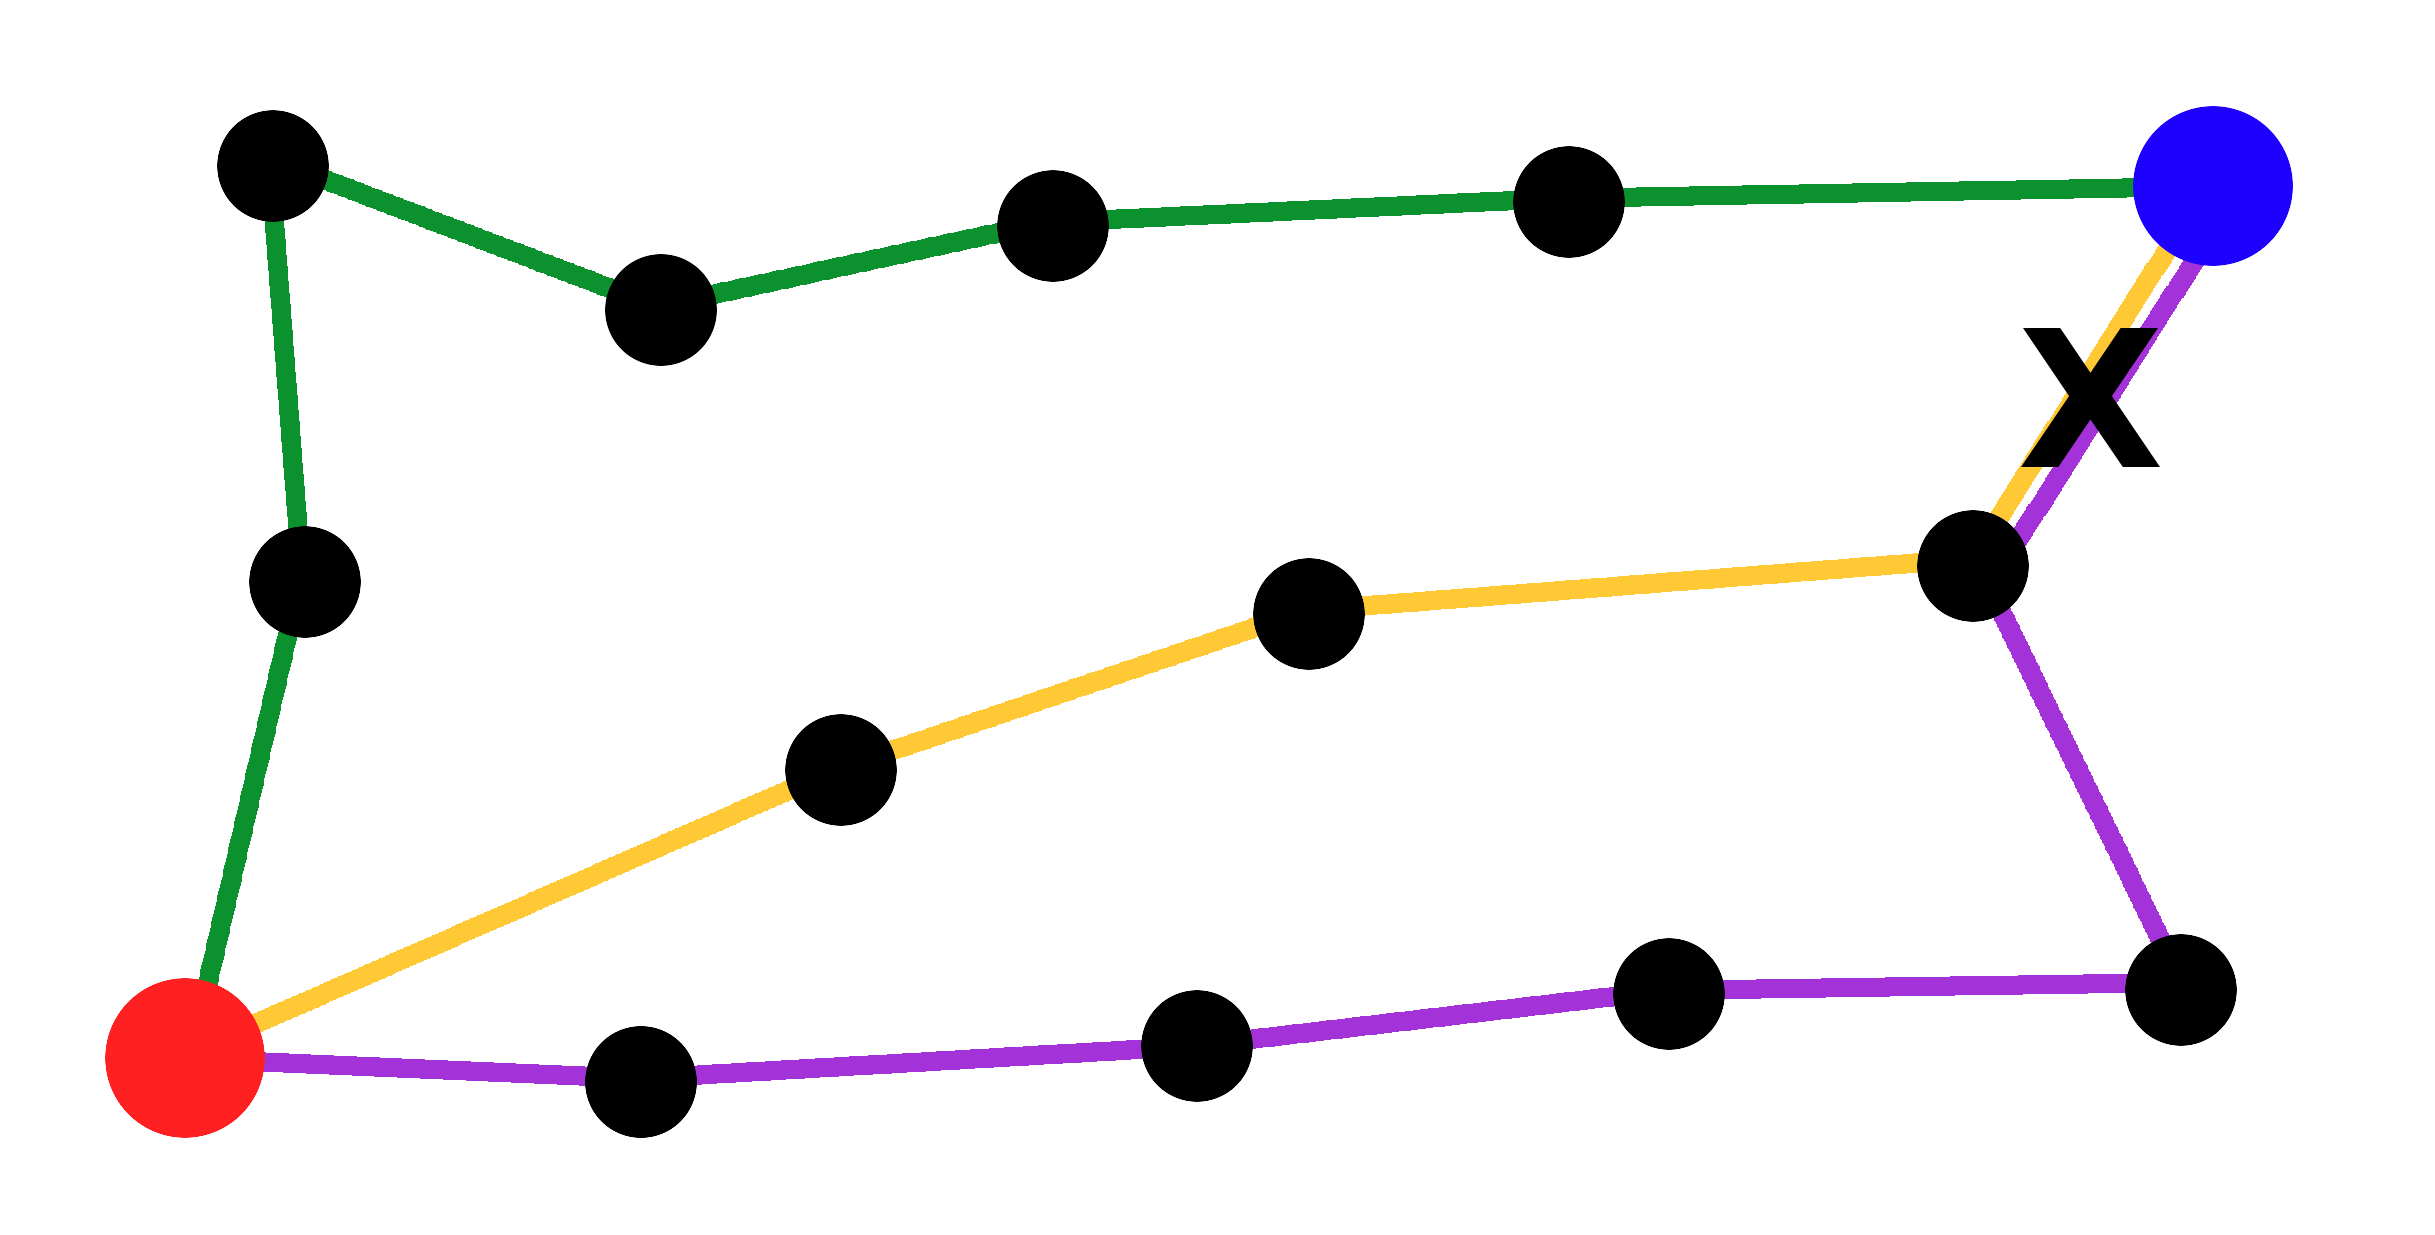
\includegraphics[width=18in]{samplefig.eps}
\end{center}
\end{textblock}



\begin{textblock}{10}(24,19)
\CHead{Getting Started}
I suggest reading this template first and getting a feel for how
the layout works.  Then, decide on the \textit{logical} formatting
of your poster -- what groupings of information do you want, and
how should they relate to one another?  Then you can start playing
around with the layout.  Keep in mind that the border and background
color options that are in this template use \texttt{pstricks} and 
thus will not play well unless you use the PostScript rendering
path.
\end{textblock}


\begin{textblock}{10}(36,04)
\CHead{Layout Details}
This template for posters creates boxes of information and then physically
places them on the poster page.  Because there is no way to tell how large
a chunk of text/images will take up, a lot of tweaking of the final layout
is required.  I think that the professional output that you get is 
worth the time invested.

The entire poster is divided into a grid of equal cell spaces.  This is
only a convenience -- boxes can be places arbitrarily within the poster,
but a coordinate system helps users organize their information.  For example,
this document uses a 46 cell wide and 26 cell tall grid.  The columns are
10 cells wide with a 2 cell spacer between columns.  To get more arbitrary
placement, you can use a finer grid or specify decimal coordinates.  The
top left corner of the poster is $(0,0)$.

Once you have made a logical division of the material that is to go into 
the poster, you can put those divisions into separate \texttt{textblock}
environments.  These have two arguments -- the width in cells and the 
position in the grid of the top left corner of the block.  You can then
place all of your blocks and move them around so that they fit in the
space provided.
\end{textblock}


\begin{textblock}{10}(36,15)
\CHead{Making a poster backup}
The \texttt{textblock} environments here transfer easily to slide
presenation packages for \LaTeX, such as \texttt{prosper}, \texttt{beamer},
and \texttt{slitex}.  Since the layout of the poster in this document is
a logical one, you can simply mimic that in your favorite slidemaking
package to obtain letter-sized sheets to use as a backup in case this
poster is is missing, damaged, incorrectly-sized, etc.

\end{textblock}


\begin{textblock}{10}(36,21)
\bibliographystyle{plain}
\bibliography{posterTemplate}
\end{textblock}



\begin{textblock}{46}(00,25.5)
\begin{center}
{\footnotesize Contact information:
Anand D.~Sarwate, 264 Cory Hall, Department of EECS, University of California, Berkeley, Berkeley, CA 94720\ \ --
Phone: 510--643--9263\ \ -- 
Email: \textit{asarwate@eecs.berkeley.edu}; 
Web: \textit{http://www.eecs.berkeley.edu/}
}
\vspace{-0.75\baselineskip}

{\footnotesize Acknowledgments: This work was performed while the
author held a National Defence Science and Engineering Graduate
Fellowship.  This template was modified only slightly from that of Ron
Kumon in order to make it more specifically a tutorial for the
Berkeley Wireless Foundations Center.}
\end{center}
\end{textblock}

\end{document}
